\documentclass[documentclass]{jsarticle}
%ディジタル信号処理 Matlab演習1
\usepackage[top=25truemm,bottom=25truemm,left=20truemm,right=20truemm]{geometry}
\usepackage{listings, jlisting, color}
\usepackage[dvipdfmx]{graphicx}
\usepackage{pdfpages}
\usepackage{amsmath}
\usepackage{amssymb, latexsym}
\usepackage{mathtools}
\usepackage{multirow}
\usepackage{color}
\usepackage{ulem}
\usepackage{here}
\usepackage{wrapfig}
\usepackage{tikz}
\usepackage{tcolorbox}
\tcbuselibrary{breakable, skins, theorems}

% 使用する関数の宣言
% (最低限これさえ宣言していれば十分だと思われるものを書いています)
\usetikzlibrary{intersections, calc, arrows, positioning, arrows.meta}


\newcommand{\Add}[1]{\textcolor{red}{#1}}
\newcommand{\Erase}[1]{\textcolor{red}{\sout{\textcolor{black}{#1}}}}
\newcommand{\ctext}[1]{\raise0.2ex\hbox{\textcircled{\scriptsize{#1}}}}

\lstset{
  basicstyle={\small},
  breaklines=true,
  frame=single,
  tabsize=3,
  numbers=left
}

\begin{document}
\title{ソフトウェア設計演習 設計演習1}
\author{222C1021 今村優希}
\maketitle

%\tableofcontents
\clearpage

\newpage

\section{今回のシステム}

今回作成対象となるシステムは「スクールバスシステム」である.
システムの仕様は以下の通りである.
一部,下記の仕様に付け加えて考えた部分があるので,その都度その機能に関して説明をする.

\begin{tcolorbox}
  利用者は、スクールバスを利用するためにチケットを購入する。
  チケットには回数券と月利用券がある。
  チケットは電子的なものであり、システムで管理し、スマホで確認可能とする。
  購入は大学生協アプリもしくはクレジットカードを使用する(どちらも外部システムを利用する)。
  スクールバスを利用する際には、乗車時と降車時にスマホをかざし記録を取る。
  スクールバスのダイヤは、大学の事務が登録し、利用者は閲覧できる。
\end{tcolorbox}

作成の流れとしては,初めにユースケース図を用いてシステムの概要を把握すると共に,機能側面からのモデル化を行った.
ある程度の概要がつかめると,静的側面からのモデル化のためにクラス図の作成を行った.
機能側面をより深めるために,最初に作成したユースケース図の記述とシーケンス図の作成をした.
最後に動的側面からモデル化するためにステートマシン図の作成を行った.

\newpage

\section{ユースケース図}

システムの概要を把握するために一番最初にユースケース図の作成を行った.
作成したユースケース図は図\ref*{fig:1-1}の通りである.
\begin{figure}[H]
  \begin{center}
    \includegraphics*[scale=0.5]{figure/1-1.png}
  \end{center}
  \caption{ユースケース図}
  \label{fig:1-1}
\end{figure}

まずは,システムの仕様から登場するアクターを設定した.
それぞれのアクターは以下のことを行う.
\begin{itemize}
  \item 利用者 
  \\スマホにログインすることで複数のことを行える
  \item 大学の事務
  \\ダイヤの登録を行う
  \item 管理者
  \\管理用にログインすることでチケットの管理を行える
  \item 外部システム
  \\チケットの購入をする際に関与する
\end{itemize}

この図を作成するにあたり難しいと思ったのは,依存関係及び汎化である.
今回は,「乗車する」と「降車する」というユースケースは「乗降の記録を取る」というユースケースに含まれている(include)と考えた.
また,「チケットの購入」と「チケットの確認」に関しては「チケットの管理をする」に含まれる(include)よう設定をした.
「チケットを管理する」というユースケースの機能に「乗降の記録を取る」という機能を付け加える(extend)という考え方をした.

スクールバスに関するアクターを作成しようかと考えたが,システムの仕様上,スクールバスに関する記述がなかったため,アクターに加えなかった.
\newpage

\section{クラス図}

ユースケース図を作成することでシステムの概要を把握できたので,そのシステムに関わるクラスの関係を作成するためにクラス図の作成を行った.
作成したクラス図は,図\ref*{fig:2-1}である.

\begin{figure}[H]
  \begin{center}
    \includegraphics*[scale=0.5]{figure/2-1.png}
  \end{center}
  \caption{クラス図}
  \label{fig:2-1}
\end{figure}

まず,考えたのは「乗客」と「管理」のクラスが「利用者」というクラスの汎化関係があるのではないかということだ.
どちらもIDやPasswordを入力してログインすることから「利用者」というクラスを継承する形で「乗客」と「管理」を結んだ.
「外部システム」と「生協アプリ」「クレジット会社」,「データベース」と「記録用「管理用」,「チケット」と「回数券」「月利用券」も同様に考えた.

「乗客」は,「ダイヤ」を見たり「スマホ」を用いたりする関係があるので,それぞれ関連を結んだ.
「スマホ」は.チケットを購入したりチケットを読み取ったりするのに使用するので,関係があるものと関連を結んだ結果が図のとおりである.

次に多重度に関して考えた.乗客と関連クラスの関係に関して考えてみる.
ダイヤ1つに対して複数の乗客が見るので,乗客の多重度が「*」であり,ダイヤが「1」である.
また,1人の乗客が1つ以上のスマホを持っていないとシステムの利用ができないので,乗客を「1」,スマホを「1...*」と設定した.
このような考えからそれぞれ多重度の設定を行った.

\newpage

\section{ユースケース記述}
作成したユースケース図(図\ref*{fig:1-1})のユースケース記述を作成した.
すべてのユースケースに対してユースケース記述を作成したが,この部分では一部のユースケースのみ考えた内容を説明する.

まずは,「乗車する」のユースケース記述を図に記載する.
\begin{figure}[H]
  \begin{center}
    \includegraphics*[scale=0.8]{figure/3-2.png}
  \end{center}
  \caption{「乗車する」のユースケース記述}
  \label{fig:3-2}
\end{figure}
乗客が乗車する際に,乗客はシステムにログインした画面をバスに設置されている読み取り機にかざすことで乗車することができる.
一方,システムはその乗車券が正しいのかを裏でチェックすることでシステムが正しく動くようにした.
また,代替系列として2-1と2-2で設定をした.
それぞれ読み取り機が読み取れなかった場合と,チケットが有効でなかった場合に動作する.

次に「チケットを購入する」のユースケースについてである.図\ref*{fig:3-4}に示している.
\begin{figure}[H]
  \begin{center}
    \includegraphics*[scale=0.8]{figure/3-4.png}
  \end{center}
  \caption{「チケットを購入する」のユースケース記述}
  \label{fig:3-4}
\end{figure}
「チケットの購入する」には,図\ref*{fig:1-1}のユースケース図のように外部システムが関わっている.
利用者が購入するチケットの種類(回数券,月利用券)を選び,その後外部システムに移動し,決済の代替を行ってもらう仕組みにした.
実際の動作はわからないが,外部システムが購入通知を出すことで当システムが購入できたと判断しチケットを保存することで購入するユースケースが完遂させるようにさせた.
そのため,代替系列では適切な選択ができなかったときと購入通知が来なかった時(外部システムで失敗したとき)のみだと判断した.

\newpage
\section{シーケンス図}
シーケンス図は,乗車用,降車用,チケット購入用の3種類作成した.
まずは,乗車用,降車用のシーケンス図を図\ref*{fig:4-1},\ref*{fig:4-2}に記載した.
\begin{figure}[H]
  \begin{center}
    \includegraphics*[scale=0.3]{figure/4-1.png}
    \caption{乗車用のシーケンス図}
    \label{fig:4-1}
    \includegraphics*[scale=0.3]{figure/4-2.png}
    \caption{降車用のシーケンス図}
    \label{fig:4-2}
  \end{center}
\end{figure}
乗車用も降車用も流れとしてはほぼ同じである.
乗客はスマホを用いることでチケットを提示し,チケット読み取り機が読み取ることで乗車することができる.
乗車用と降車用で異なるのはシステム内での動作で,乗車用では記録用DBが管理用DBに対して読み取ったチケットが有効であるかを確認する.
有効であった場合に乗車音を出すことで乗客は乗車することが可能である.
一方,降車用では記録用DBが管理用DBに通知をしてチケットの更新を行うのみで,管理用DBから記録用DBに対しての動作はない.
また,代替系列もそれぞれ設定した.

次に購入用のシーケンス図である.
図\ref*{fig:4-3}に示した.
購入用では,2種類ある回数券を選択をさせた後に管理用DBが記録を行い,その後外部システムに支払いを対応してもらうようにしている.
支払いが完了したら,外部システムから管理用DBに通知が行き,利用者の手元のスマホにチケットが表示させる設計にした.
代替系列では,適切な選択ができなかった時,外部システムから通知が来なかった場合で考えた.それぞれエラーをスマホ上に通知することで代替系列の対処を行った.
\begin{figure}[h]
  \begin{center}
    \includegraphics*[scale=0.4]{figure/4-3.png}
  \end{center}
  \caption{チケット購入用のシーケンス図}
  \label{fig:4-3}
\end{figure}

\newpage

\section{ステートマシン図}
作成したステートマシン図は「回数券」「月利用券」「スマホ」の3種類である.

回数券のステートマシン図は図\ref*{fig:5-1}である.
チケットを購入すると使用待機中に遷移する.
乗降を持って1回の使用が終わり,そこで残りの回数が0回か1回以上かで取りうる状態が異なるよう設計した.

月利用券のステートマシン図は図\ref*{fig:5-2}である.
月利用券は,定期券と同じで使用期間が設定されているという判断をした.
使用待機中から使用できるのは,使用期限以内に設定し,期限が切れると同時に「期限切れ」に状態が遷移する.
\begin{figure}[h]
  \centering
  \begin{minipage}[b]{0.49\columnwidth}
      \centering
      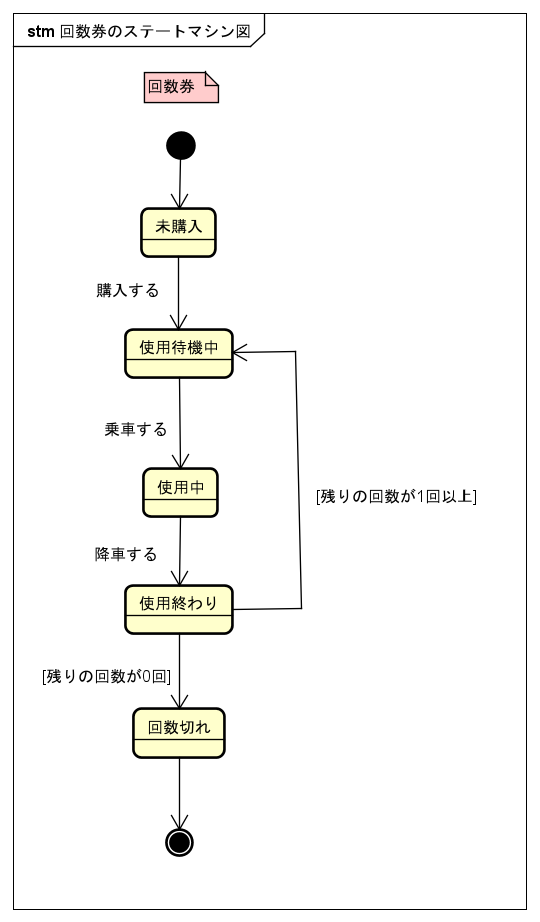
\includegraphics[width=0.9\columnwidth]{figure/5-1.png}
      \caption{回数券のステートマシン図}
      \label{fig:5-1}
  \end{minipage}
  \begin{minipage}[b]{0.49\columnwidth}
      \centering
      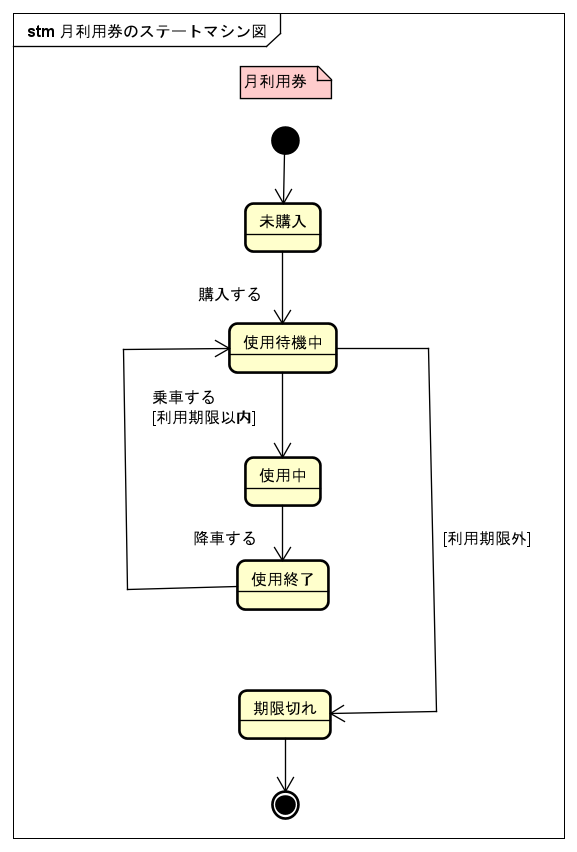
\includegraphics[width=0.9\columnwidth]{figure/5-2.png}
      \caption{利用券のステートマシン図}
      \label{fig:5-2}
  \end{minipage}
  \end{figure}

次に,スマホのステートマシン図を図\ref*{fig:5-3}に示している.
ユースケース図やクラス図から,スマホはログインした後にチケットをかざしたり,購入,確認という行為を行える.
この考えから,「ログイン」という状態に,「チケット」や「購入」という状態が含まれるという形で設定をした.
「購入」に関しては,外部システムを利用するのでそのように設計をした.
戻るボタンを押下することで「ホーム」状態に戻るようにした.
\begin{figure}[H]
  \begin{center}
    \includegraphics*[scale=0.5]{figure/5-3.png}
  \end{center}
  \caption{スマホのステートマシン図}
  \label{fig:5-3}
\end{figure}

\section{まとめ}
今回の設計演習ではユースケース図を作成することでそのクラス図の作成がうまく行った.
ユースケース図に関してはかなりの時間を費やして設計を行った.
includeやextendの扱い方に関しては少々悩んだ.
また,「スマホでログインする」から様々なことを行えるという設計は工夫した点である.

クラス図に関しては,今回のシステムで登場するものを書いて関連を結んだだけである.
しかし,汎化関係に関しては悩んだ部分である.

シーケンス図では,作成したユースケース記述を元に作成を行った.
ここで「管理用DB」と「記録用DB」の2つのクラスを作成しようと考えた.

ステートマシン図では,スマホの状態遷移を工夫した.
ログイン状態で複数のことを行うので,ログイン状態に複数の状態を含むという点を工夫した.

\end{document}